%%%%%%%%%%%%%%%%%%%%%%%%%%%%%%%%%%%%%%%
% Shrikant - One Page Two Column Resume
% IMPORTANT: THIS TEMPLATE NEEDS TO BE COMPILED WITH XeLaTeX
%
% This template uses several fonts not included with Windows/Linux by
% default. If you get compilation errors saying a font is missing, find the line
% on which the font is used and either change it to a font included with your
% operating system or comment the line out to use the default font.
% 
%%%%%%%%%%%%%%%%%%%%%%%%%%%%%%%%%%%%%%
% 
% TODO:
% 1. Integrate biber/bibtex for article citation under publications.
% 2. Figure out a smoother way for the document to flow onto the next page.
% 3. Add styling information for a "Projects/Hacks" section.
% 4. Add location/address information
% 5. Merge OpenFont and MacFonts as a single sty with options.

\documentclass[]{shrikant-resume-openfont}
\usepackage{fancyhdr}
\usepackage{graphicx}
 
\pagestyle{fancy}
\fancyhf{}
 
\begin{document}

%%%%%%%%%%%%%%%%%%%%%%%%%%%%%%%%%%%%%%
%
%     LAST UPDATED DATE
%
%%%%%%%%%%%%%%%%%%%%%%%%%%%%%%%%%%%%%%
\lastupdated

%%%%%%%%%%%%%%%%%%%%%%%%%%%%%%%%%%%%%%
%
%     TITLE NAME
%
%%%%%%%%%%%%%%%%%%%%%%%%%%%%%%%%%%%%%%
\namesection{Shrikant}{Mali}{
+47 96014328 | \href{mailto:shrikant.b.mali@gmail.com}{shrikant.b.mali@gmail.com}}

%%%%%%%%%%%%%%%%%%%%%%%%%%%%%%%%%%%%%%
%
%     COLUMN ONE
%
%%%%%%%%%%%%%%%%%%%%%%%%%%%%%%%%%%%%%%

\begin{minipage}[t]{0.33\textwidth} 

%%%%%%%%%%%%%%%%%%%%%%%%%%%%%%%%%%%%%%
%     LINKS
%%%%%%%%%%%%%%%%%%%%%%%%%%%%%%%%%%%%%%
\section{Photo}
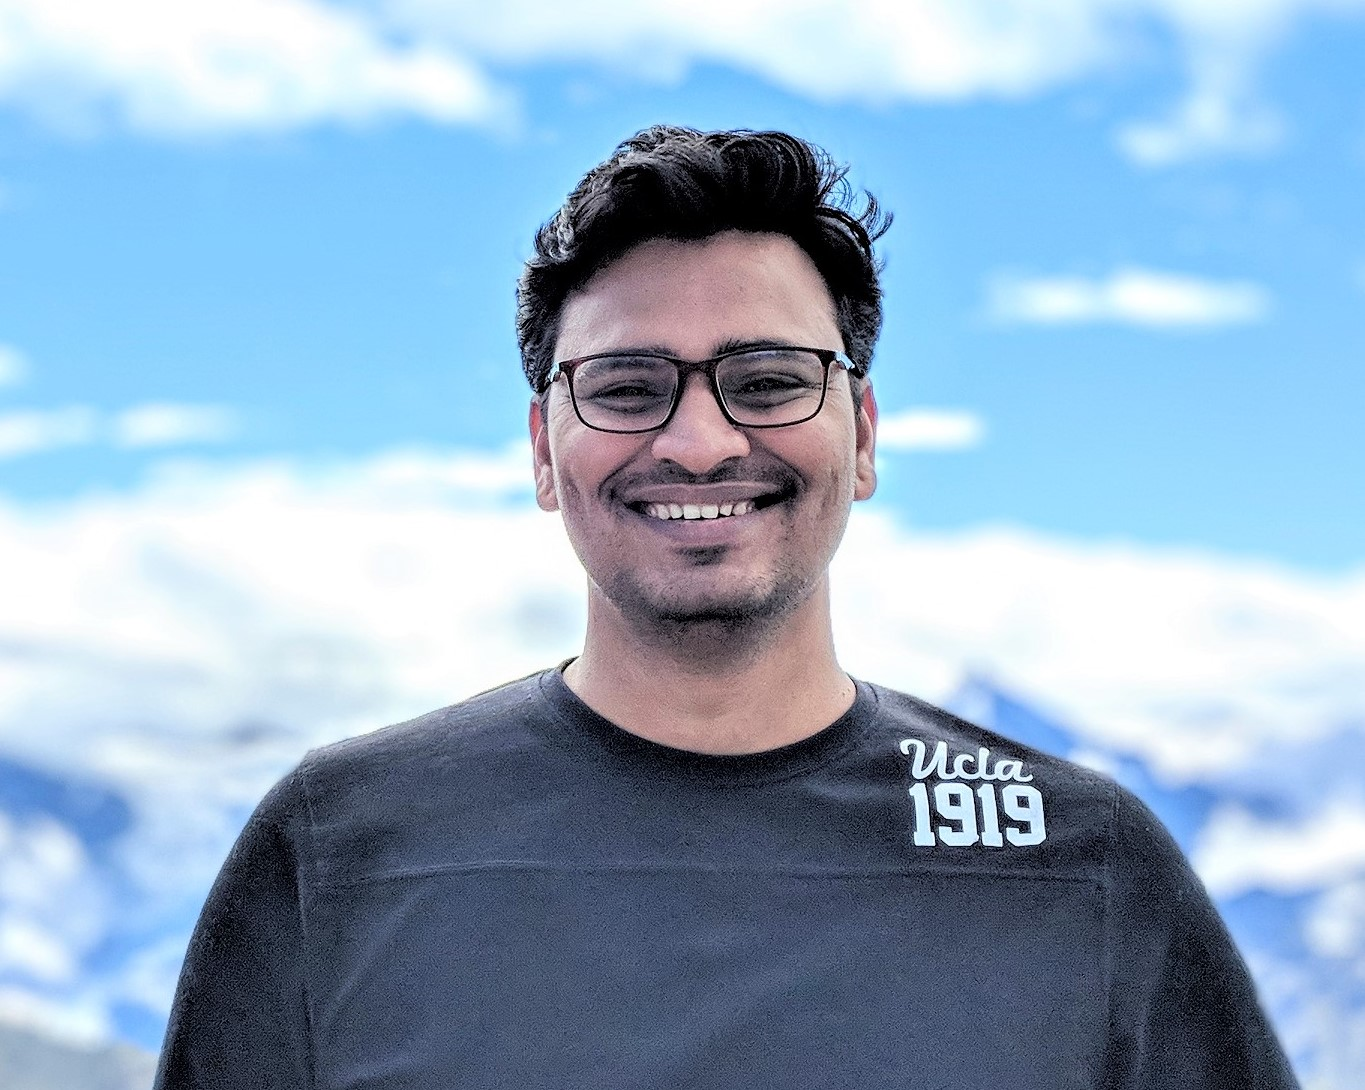
\includegraphics[height=4cm]{photo.jpg} \\

\section{Links} 
Github:// \href{https://github.com/shrikantbmali}{\bf shrikantbmali} \\
LinkedIn://  \href{https://www.linkedin.com/in/shrikantmali/}{\bf shrikantmali} \\
Twitter://  \href{https://twitter.com/shribmali}{\bf @shribmali} \\


%%%%%%%%%%%%%%%%%%%%%%%%%%%%%%%%%%%%%%
%     SKILLS
%%%%%%%%%%%%%%%%%%%%%%%%%%%%%%%%%%%%%%
\section{Skills}
\vspace{1mm}
\textbullet{} C\# \textbullet{} Xamarin \textbullet{} .net Core
\textbullet{} WPF \textbullet{} WF.\\
\vspace{1mm}
\textbullet{} TDD \textbullet{} Design Patterns \textbullet{} OOP\\ 
\vspace{1mm}
\textbullet{} REST \textbullet{} Azure DevOps 
\textbullet{} Agile \textbullet{} SAFe\\
\vspace{1mm}
\textbullet{} Git \textbullet{} VS \textbullet{} VSCode \textbullet{} WireShark \\
\vspace{1mm}
\textbullet{} Asp.net \textbullet{} JavaScript \textbullet{} TypeScript\\
\vspace{1mm}
\textbullet{} HTML \textbullet{} Angular \textbullet{} Ionic \textbullet{} Cordova\\
\vspace{1mm}
\textbullet{} github actions \textbullet{} Jenkins

\vspace{\topsep}

\location{Beginner:}
\vspace{1mm}
\textbullet{} DOCKER \textbullet{} Microservice Architecture\\
\vspace{1mm}
\textbullet{} CSS \textbullet{} Apache Thrift \textbullet{} Raspberry Pi\\
\vspace{1mm}
\textbullet{} Google Protobuf

\vspace{\topsep}

%%%%%%%%%%%%%%%%%%%%%%%%%%%%%%%%%%%%%%
%     Certifications
%%%%%%%%%%%%%%%%%%%%%%%%%%%%%%%%%%%%%%

\section{Notable Mentions}
\vspace{1mm}
\subsection{Side Projects}
\vspace{1mm}
\textbullet{} JSBridge: A Bridge between dotnet and Javascript.\\
\vspace{1mm}
\textbullet{} Light MVVM Lib. for fast and Clean Development.\\
\vspace{1mm}
\textbullet{} Server Endpoint for IOT devices using Raspberry Pi.\\
\sectionsep

\subsection{Certifications}
\vspace{1mm}
\textbullet{} Fluent API \\
\vspace{1mm}
\textbullet{} SAFe 4.0 Certification. \\

%%%%%%%%%%%%%%%%%%%%%%%%%%%%%%%%%%%%%%
%
%     COLUMN TWO
%
%%%%%%%%%%%%%%%%%%%%%%%%%%%%%%%%%%%%%%

\end{minipage} 
\hfill
\begin{minipage}[t]{0.66\textwidth} 

%%%%%%%%%%%%%%%%%%%%%%%%%%%%%%%%%%%%%%
%     EXPERIENCE
%%%%%%%%%%%%%%%%%%%%%%%%%%%%%%%%%%%%%%
\section{About}
\vspace{\topsep}
\begin{tightemize}
\item A Bachelor in Computer Engineering
\item Eight+ Years of experience in Microsoft Stack, Xamarin, Angular and Cordova.
\item Strong understanding of OOP and Design patterns.
\item A Full-Stack and Cloud development aspirant.
\end{tightemize}
\sectionsep

\section{Experience}
\runsubsection {Admincontrol}\descript{| App Development team lead. }
\location{Nov 2020 - Present | Drammen, Norway}
\begin{tightemize}
\item Responsible for Planning and Deliveries of the Cross platform application.
\item Managing Deployment and Releases of the apps.
\item Team Coordination.
\end{tightemize}
\sectionsep

\runsubsection {SIEMENS}\descript{| Senior Software Engineer \& Team Leader }
\location{May 2014 - Sep 2020 | Pune, MH}
\begin{tightemize}
\item Responsible for Design, Develop and Delivery of Mobile Applications.
\item Implemented multiple Mobile application using Xamarin and Angular for Both Android and iOS
\item ASP.net Core Developed a Time and Space efficient queryable Microservice to fetch data from IOT devices.
\item Implemented a REST Api using ASP.net Core as a backend for mobile application.
\item Developed a framework which allows Xamarin application to have HTML UI (Android, iOS, Winodws)
\item Implemented a Yeoman Generator generate Xamarin-Angular hybrid application.
\item Created CI/CD for Xamarin(android, iOS), Cordova(android, iOS), on Git-Lab, Jenkins.
\item Committee member: Inner Sourcing, Digitization.
\end{tightemize}
\sectionsep

\runsubsection{QuicSolv}
\descript{| Software Developer }
\location{Dec 2013 – April 2014 | Pune, MH}
\vspace{\topsep} % Hacky fix for awkward extra vertical space
\begin{tightemize}
\item Worked on a Windows Forms POS Application for US pharma industries.
\item Developed a file based order and invoice communication infrastructure.
\end{tightemize}
\sectionsep

\runsubsection{WebTech Developers}
\descript{| Software Developer }
\location{March 2012 – Dec 2013 | Pune, MH}
\begin{tightemize}
\item Worked on multiple IP and USB Security Cameras monitoring tools.
\item Implemented non-linear Range scale to change the degree of image detection based to value selected.
\item Design and developed a scalable and dynamic timeline based Media Played which showed recorded media on timeline based on the time and length.
\item Worked on Frame Analyzer to detect movement.
\end{tightemize}
\sectionsep

%%%%%%%%%%%%%%%%%%%%%%%%%%%%%%%%%%%%%%
%     AWARDS
%%%%%%%%%%%%%%%%%%%%%%%%%%%%%%%%%%%%%%

\section{Awards} 
\begin{tabular}{rll}
2014	 & Runner up & Hackathon (Meeting Room Occupancy detector)\\
2015	 & Nomination & Star Performer of the year\\
2017	 & Winner & Hackathon (Building Engg. using Hololens)\\
2018     & Intellectual Property & Filed Patent for Building Engg. with VR\\
2014-2019 & Additional Awards & 4 High Performer, 1 Key Resource and 1 SPOT\\
\end{tabular}
\sectionsep

\end{minipage} 
\end{document}  \documentclass[]{article}
